% !TEX root = ../main.tex
\section{Trabalho Desenvolvido em Contexto de Laboratório e Modelação CAD}
\label{sec:laboratorio}

Durante o mês de julho de 2026, em regime presencial, as atividades desenvolvidas incidiram sobre o enquadramento experimental e, primordialmente, sobre a modelação tridimensional assistida por computador em CAD (SolidWorks\textregistered), integração mecânica de novos subsistemas e preparação da bancada experimental dedicada ao estudo de fenómenos de escoamento em ebulição (\emph{flow boiling}) com fluidos de trabalho orgânicos e água. Esta fase constituiu uma etapa basilar de engenharia mecânica aplicada, articulando conceitos de conceção mecânica, termodinâmica, transmissão de calor, hidráulica e metrologia experimental nos laboratórios de energias da ADAI e do Departamento de Engenharia Mecânica da Universidade de Coimbra.

O escoamento em ebulição no interior de condutas representa um dos processos convectivos de maior eficácia na transferência de calor, assumindo papel preponderante em permutadores compactos, sistemas de arrefecimento de elevada densidade térmica e ciclos termodinâmicos de Rankine com fluido orgânico (ORC) vocacionados para a recuperação de calor residual industrial e captura criogénica de carbono no projeto Bio-Waste\textsubscript{2}Carbon. A compreensão e caracterização quantitativa destes regimes de escoamento exigem instalações experimentais rigorosamente concebidas, estáveis e dotadas de acesso ótico de alta precisão.

\subsection{Enquadramento da Instalação Experimental e Componentes da Bancada}
\label{subsec:concecao_bancada}

A bancada experimental do projeto BW2C foi concebida para viabilizar ensaios termohidráulicos controlados sob uma ampla gama de caudais mássicos ($G$), títulos de vapor ($x$), fluxos de calor impostos ($q''$) e pressões de saturação ($P_{\text{sat}}$). A instalação opera em circuito fechado, garantindo a contenção estanque e a recirculação contínua do fluido de trabalho orgânico. Na \autoref{fig:bancada_render} apresenta-se o modelo tridimensional global da bancada experimental com a identificação dos seus componentes funcionais principais.

\begin{figure}[!htbp]
    \centering
    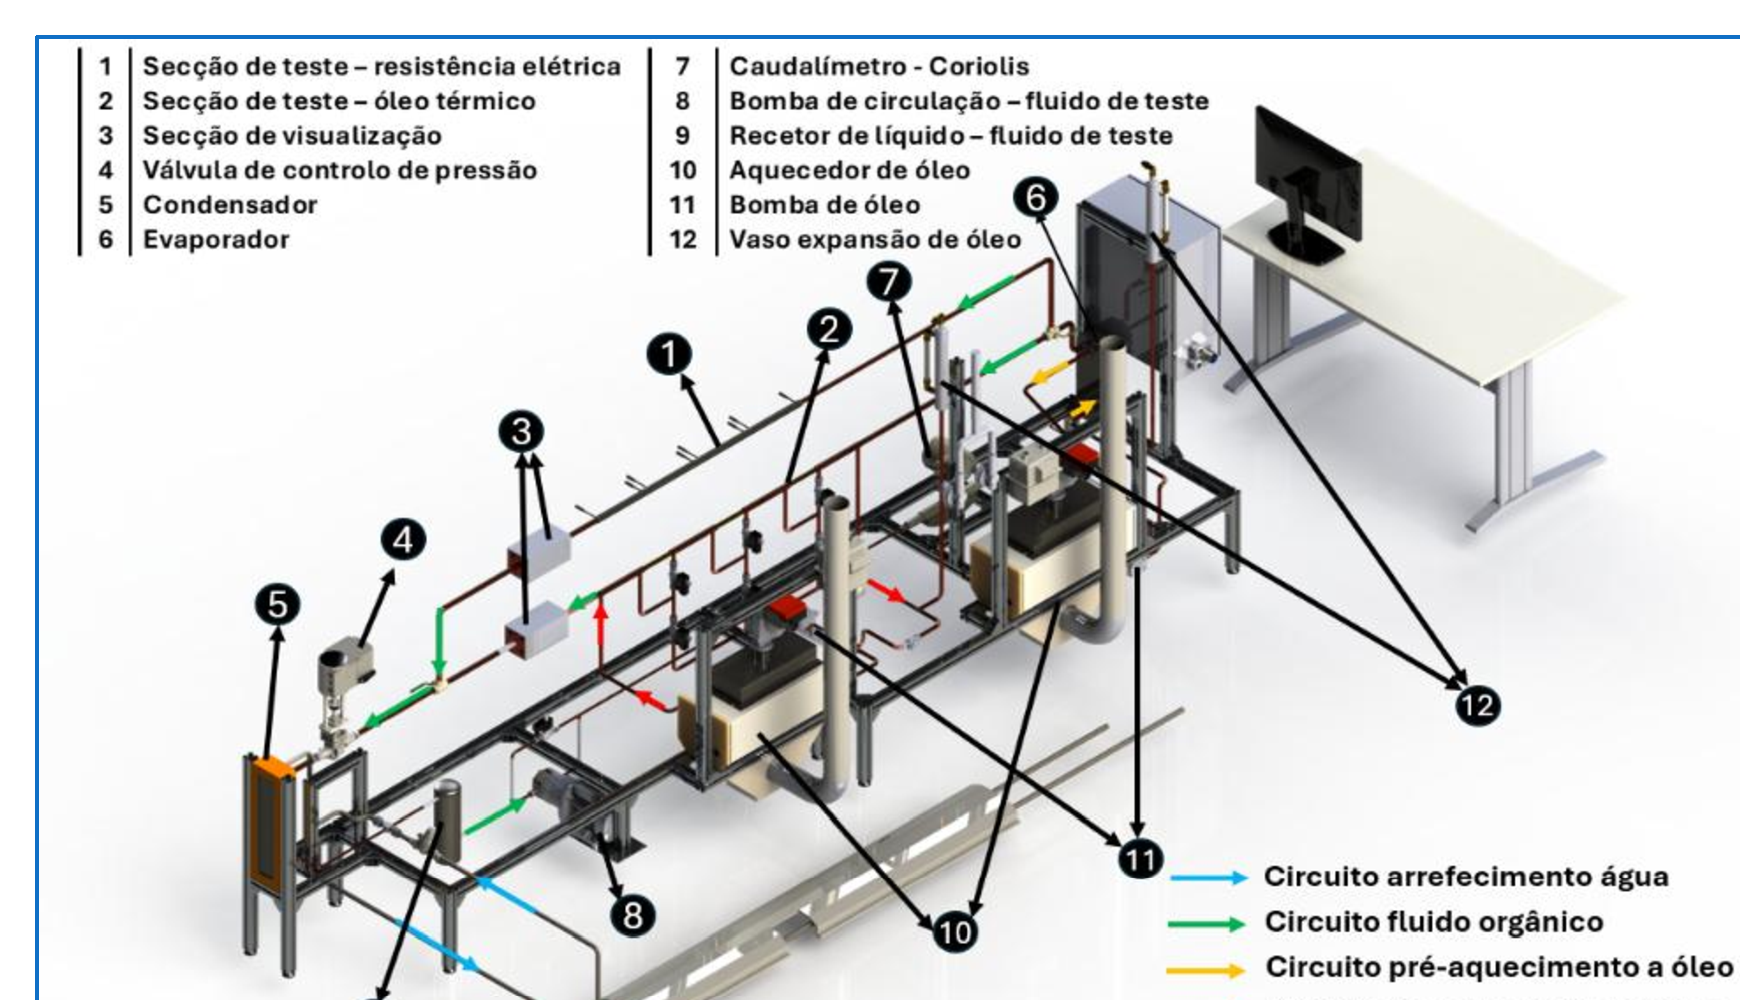
\includegraphics[width=0.92\textwidth]{assets/fig1_bancada_render.png}
    \caption{Render tridimensional da bancada experimental para estudo de escoamentos em ebulição (ADAI / UC).}
    \label{fig:bancada_render}
\end{figure}

A arquitetura geral da instalação é estruturada em torno de múltiplos subsistemas complementares:
\begin{itemize}
    \item \textbf{Circuito principal de escoamento do fluido de teste (verde na \autoref{fig:bancada_render}):} Condutas em aço inoxidável e cobre com diâmetros normalizados, integrando a bomba de recirculação magnética (item 8), o tanque recetor de líquido (item 9), secções de aquecimento, a secção de visualização transparente (item 3) e o condensador (item 5);
    \item \textbf{Secção de teste e aquecimento primário (itens 1 e 2):} Módulos térmicos dedicados ao fornecimento uniforme de fluxo de calor para indução de ebulição, com secção tubular aquecida por resistências elétricas calibradas e secção alimentada por permutador de óleo térmico;
    \item \textbf{Secção de visualização ótica transparente (item 3):} Tubo de vidro borossilicato de alta transparência ótica com diâmetro interno nominal $D_i = 20{,}0\,\mathrm{mm}$ e diâmetro externo $D_o = 26{,}0\,\mathrm{mm}$, permitindo a observação direta dos regimes de escoamento (bolhas dispersas, \emph{slugs}, transições anulares);
    \item \textbf{Circuito secundário de óleo de aquecimento (amarelo/vermelho na \autoref{fig:bancada_render}):} Compreende a bomba de circulação de óleo térmico (item 11), o aquecedor de óleo (item 10) e o vaso de expansão atmosférico/pressurizado (item 12), assegurando a regulação precisa da temperatura do óleo;
    \item \textbf{Circuito de arrefecimento e condensação (azul na \autoref{fig:bancada_render}):} Circuito de água de refrigeração ligado ao condensador de placas/tubular (item 5), responsável pela condensação total do vapor gerado e pelo subarrefecimento do fluido antes da sua recirculação;
    \item \textbf{Sistema de controlo de pressão e expansão:} Válvula reguladora de pressão motorizada (item 4), instalada a jusante da secção de ensaio, que atua na linha de retorno para estabilização da pressão operacional de saturação do ciclo;
    \item \textbf{Instrumentação e aquisição de dados:} Caudalímetro mássico de Coriolis de elevada precisão (item 7), transmissores de pressão diferencial e absoluta, e matrizes axiais e perimétricas de termopares tipo K conectadas a módulos compactos de aquisição National Instruments (NI).
\end{itemize}

\subsection{Modelação Tridimensional em CAD (SolidWorks\textregistered) e Integração Mecânica}
\label{subsec:cad_solidworks}

No decurso das atividades de julho de 2026, a principal intervenção técnica desenvolvida pelo autor concentrou-se na modelação tridimensional assistida por computador em SolidWorks\textregistered{}, com o objetivo de compatibilizar, atualizar e aperfeiçoar o projeto mecânico da bancada experimental perante novas necessidades operacionais e instrumentais da equipa de investigação.

A modelação paramétrica e a verificação tridimensional foram orientadas segundo quatro vertentes fundamentais:

\subsubsection{Integração do Tanque Recetor de Líquido (\emph{Liquid Receiver})}
\label{subsubsec:cad_liquid_receiver}

A estabilidade operacional de circuitos fechados de escoamento bifásico depende criticamente da manutenção de uma alimentação monofásica líquida estável na admissão da bomba de recirculação. A presença de bolsas de vapor arrastadas ou de oscilações bruscas de pressão pode conduzir a fenómenos severos de cavitação, degradação do caudal mássico e danos no impulsor magnético.

Por forma a mitigar estes riscos, procedeu-se à modelação e integração mecânica no modelo global em SolidWorks\textregistered{} do tanque recetor de líquido (\emph{liquid receiver}, identificado pelo item 9 na \autoref{fig:bancada_render}). O trabalho compreendeu:
\begin{enumerate}
    \item Definição do posicionamento espacial ótimo do reservatório na secção inferior da bancada, maximizando a carga hidrostática positiva disponível sobre a bomba (\emph{Net Positive Suction Head} -- NPSH);
    \item Modelação das ligações flangeadas e roscadas com as linhas de retorno de líquido arrefecido provenientes do condensador;
    \item Confeção e posicionamento de elementos de fixação mecânica estrutural aos perfis modulares de alumínio da bancada, garantindo amortecimento de vibrações e fácil acesso visual para verificação do nível de fluido.
\end{enumerate}

\subsubsection{Reconfiguração Estrutural e Elevação da Válvula Reguladora de Pressão}
\label{subsubsec:cad_valvula_pressao}

A válvula de regulação e controlo de pressão da bancada (item 4 na \autoref{fig:bancada_render}) desempenha um papel determinante na fixação do ponto termodinâmico de saturação durante os ensaios de escoamento ebulitivo. Contudo, na configuração geométrica preliminar da instalação, a válvula encontrava-se sujeita a desníveis espaciais e constrangimentos de acessibilidade para acoplamento do atuador motorizado.

O autor concebeu e modelou no SolidWorks\textregistered{} a reconfiguração estrutural do suporte da válvula:
\begin{enumerate}
    \item Modelação de uma subestrutura elevada em perfis estruturais modulares de alumínio extrudido, rigidamente acoplada à armação principal da bancada através de cantoneiras e parafusos com porca em T;
    \item Elevação geométrica da base da válvula até à cota horizontal exata das linhas de escoamento a jusante da secção de visualização, eliminando cotovelos e desvios desnecessários que geravam perdas de carga singulares indesejadas;
    \item Garantia de espaço livre circundante para manobra, instalação da cablagem de alimentação do servomotor e intervenções de manutenção periódica.
\end{enumerate}

\subsubsection{Roteamento e Alinhamento Tridimensional das Tubagens do Circuito}
\label{subsubsec:cad_tubagens}

A introdução do novo tanque recetor e a elevação da válvula de controlo exigiram a reformulação e o alinhamento das tubagens do circuito hidráulico fechado. Recorrendo às ferramentas avançadas de encaminhamento tridimensional (\emph{Routing}) do SolidWorks\textregistered{}, efetuou-se:
\begin{enumerate}
    \item Deteção e resolução de colisões e interferências geométricas (\emph{clash detection}) entre as tubagens do fluido orgânico, as linhas de óleo térmico de pré-aquecimento e as condutas de água fria do condensador;
    \item Otimização dos comprimentos lineares de tubo e garantia dos raios de curvatura mínimos admissíveis para condutas de cobre e aço inoxidável, prevenindo estrangulamentos de secção e tensões residuais mecânicas;
    \item Verificação do espaçamento perimétrico de segurança e acessibilidade ergonómica para instrumentação, sensorização perimétrica e manutenção das linhas de fluido;
    \item Posicionamento das tomadas de pressão e mangas para termopares nas zonas retilíneas a montante e a jusante dos pontos de transição, respeitando as normas de metrologia hidrodinâmica (comprimentos de desenvolvimento hidráulico mínimos $L/D \ge 10$).
\end{enumerate}

\subsubsection{Interface Mecânica e Alinhamento da Secção de Ensaio Ótica}
\label{subsubsec:cad_seccao_otica}

A preparação do desafio central de visão computacional e inteligência artificial exigiu especial atenção à secção transparente de visualização (item 3 na \autoref{fig:bancada_render}). O autor procedeu à verificação dimensional rigorosa dos apoios do tubo em vidro borossilicato ($D_i = 20{,}0\,\mathrm{mm}$), garantindo:
\begin{enumerate}
    \item Perfeito alinhamento coaxial entre as extremidades da conduta de vidro e os troços adjacentes metálicos da bancada, evitando descontinuidades de bordo ou degraus internos que pudessem induzir perturbações no escoamento ou promover pontos de nucleação espúrios antes da janela de observação;
    \item Definição do suporte estrutural livre de vibrações mecânicas para a câmara de alta velocidade e para a fonte de retroiluminação colimada com lente corretiva cilíndrica externa;
    \item Estabelecimento das dimensões espaciais exatas do campo de visão (\emph{Field of View} -- FOV), que serviram de referência física absoluta para a posterior calibração métrica pixel-a-metro desenvolvida na etapa computacional.
\end{enumerate}

\subsection{Síntese da Fase Laboratorial e de Modelação}
\label{subsec:sintese_laboratorio}

A etapa de trabalho presencial realizada em julho de 2026 permitiu consolidar a arquitetura mecânica da bancada experimental através da modelação integrada em SolidWorks\textregistered{}. A integração bem-sucedida do tanque recetor de líquido, a elevação da estrutura da válvula de pressão e o alinhamento geométrico rigoroso das tubagens e da secção ótica de ensaios asseguraram a consistência física e dimensional da instalação. 

Este trabalho de base forneceu os parâmetros geométricos determinantes (geometria interna circular de $20{,}0\,\mathrm{mm}$, alinhamento axial e características do campo de visão) indispensáveis para alimentar com rigor físico os algoritmos de segmentação semântica por inteligência artificial, reconstrução tridimensional com confinamento cordal e cinemática de alta velocidade implementados na fase subsequente em Python.
